\section{GUI}
\label{sec:Gui}
\subsection{Bakgrunn}
GUI, graphical user interface, er et grensesnitt som lar brukerne samhandle med et dataprogram grafisk, vanligvis ved hjelp av tastatur og datamus. I motsetning til typiske shellapplikasjoner hvor man navigerer ved hjelp av kommandoer, består et grafiske grensesnittet ofte av grafiske ikoner og lydindikatorer.\cite{wiki:GUI} Grunnet den bratte læringskurven på en kommandobasert datamaskin med shellapplikasjoner ble grafisk brukergrensesnitt med mulighet for å bruke mus til å klikke på knapper, tekstfelt og informasjonsfelt raskt populært. Hos de to mest populære operativsystemene på markedet i dag, Windows og MacOS, er det GUI-et står i sentrum, mens det i UNIX er det mer en blanding av et kommandobasert system og grafisk brukergrensesnitt.

Vi ønsket at det skulle være lettere å benytte seg våre implementasjoner nevnt fra kapittel \ref{sec:Glatting} - \ref{sec:Anonymisering}, og bestemte oss for å lage vårt eget program med et grafisk brukergrensesnitt. Her skal det være mulighet for å utføre alle de implementerte operasjonene interaktiv på ulike utvalgte bilder. Vi endte opp med å bruke det foreslåtte rammeverket \texttt{PyQt5}\footnote{\url{https://pypi.org/project/PyQt5/}}, som gjør det enkelt å bruke implementasjonene skrevet vi allerede hadde skrevet med Python i GUI-applikasjonen. Ved å skrive programmet i PyQt5 kan man kjøre programmet på både Windows, MacOS og Linux, noe som gjør at vi forminsker arbeidsmengden betraktelig.

\subsection{Implementasjon}
Programmet kjøres fra \texttt{Main.py} hvor main ligger. Vi har valgt en vindusbasert applikasjon hvor man fra hjemskjermen kan velge hvilken implementasjon man har lyst til å benytte seg av. Vi har funnet det hensiktsmessig å dele applikasjonen opp i ulike moduler, hvor det er en modul for hjemskjermen og en modul for hver av implementasjonene. Hver modul har sin egen .py-fil i mappa \texttt{src/GUI} hvor all kode er lagret. Dette har vi gjort for god organisering ved å skille de ulike modulene i applikasjonen fra hverandre. Det er også mer oversiktelig når vi importerer de ulike bibliotekene vi har bruk for i den aktuelle modulen. 

På grunn av at vi har valgt en vindusbasert applikasjon har vi derfor laget et design for hver modul. Designet til hver modul lagres som en .ui-fil som importeres når en modul initialiseres. Designet er gjort i \texttt{Qt5 Designer}\footnote{\url{https://pypi.org/project/PyQt5Designer/}}, som gjør det enkelt å lage et oversiktelig UI med tekstfelter, knapper og bilder. Alle .ui-filene er lagret i mappa \texttt{src/GUI/UI}. Hver gang Main.py lastes tilpasses applikasjonen slik at den oppfører seg likt på skjermer med ulik pikseltetthet.

\begin{lstlisting}[language=Python]
QtWidgets.QApplication.setAttribute(QtCore.Qt.AA_EnableHighDpiScaling,True)
QtWidgets.QApplication.setAttribute(QtCore.Qt.AA_UseHighDpiPixmaps,True)
\end{lstlisting}

Når en modul initialiseres må vinduets dimensjoner justeres. Dette må gjøres fordi designet er laget med Qt5 Designer, og oppfører seg derfor annerledes på skjermer med ulike dimensjoner. Disse justeringene gjøres ved hjelp av funksjonen adjustScreen(). Her får man dimensjonen ved å hente skjermens høyde og bredde, og bruker denne til å justere vinduet. Hvert vindu er forskjellig fra hverandre, og derfor har hver modul sin egen adjustScreen() funksjon.

\begin{lstlisting}[language=Python]
def adjustScreen(self):
    screenWidth = app.primaryScreen().size().width()
    screenHeight = app.primaryScreen().size().height()
    if screenWidth/screenHeigh == 1.5:
        width = int(screenWidth / 1.8)
        height = int(screenHeight / 2)
    else:
        width = int(screenWidth / 2.22222)
        height = int(screenHeight / 1.95298)
    self.setGeometry(500, 80, width, height)
\end{lstlisting}

Hjemskjermen består av et antall knapper med tilhørende tekst som forklarer hva den aktuelle implementasjonen gjør. Når man klikker på en knapp opprettes en dialog til denne modulen. Hvis det lykkes med å opprette en dialog vil et nytt vindu åpnes hvor den aktuelle modulens design og funksjonaliteter vises. 

Hovedelementet i hver modul er bildet som man ser i (figur \ref{fig:guiexample}) Vi har valgt å bruke MatPlotLib til å vise bilder. Dette gjør at vi kan bruke \texttt{plt.imshow()}\footnote{\url{https://matplotlib.org/3.2.1/api/_as_gen/matplotlib.pyplot.imshow.html}} som vi har brukt i hver enkelt implementasjon i Jupyter Notebook-filene. I vår applikasjon er dette en bedre metode å vise bilder på sammenliknet med alternativet hvor vi da ville brukt QLabel og \texttt{setPixMap}\footnote{\url{https://doc.qt.io/archives/qt-4.8/qlabel.html#pixmap-prop}}. Selve bildet er et imagewidget av typen FigureCanvas, og vi har derfor opprettet en egen klasse \texttt {imagewidget} i filen \texttt{src/imagewidget}. Ved oppstart av hver modul initialiseres imagewidget hvor \texttt{self.img} opprettes og initialiseres. Hver gang et nytt bilde skal vises kalles \texttt{showImage(self, image, colour=True)}. Her blir det lagt til subplot, aksene fjernes og bildet justeres slik at det fyller mest mulig av bilderammen. Avhengig av om colour er True eller False, vises enten et fargebilde eller et gråtonebilde ved bruk av imshow(). Det er i hver modul lagret \texttt{self.path} som hele tiden er oppdatert med filstien til bilde som er valgt. Denne benyttes når brukeren vil se annet bilde eller ta bort effekten gjort på bildet og vise originalbildet. Hver modul har også en lokal variabel \texttt{self.image} hvor det bildet som vises i applikasjonen ligger lagret som en numpy array. Denne brukes når brukeren vil lagret bildet, hvor den sendes til \texttt{FunctionGUI/saveImage}. Her åpnes en \texttt{QFileDialog}\footnote{\url{https://doc.qt.io/qt-5/qfiledialog.html}}, som returnerer ønsket navn på filen og filsti til ønsket mappe.

\begin{figure}
\begin{center}
    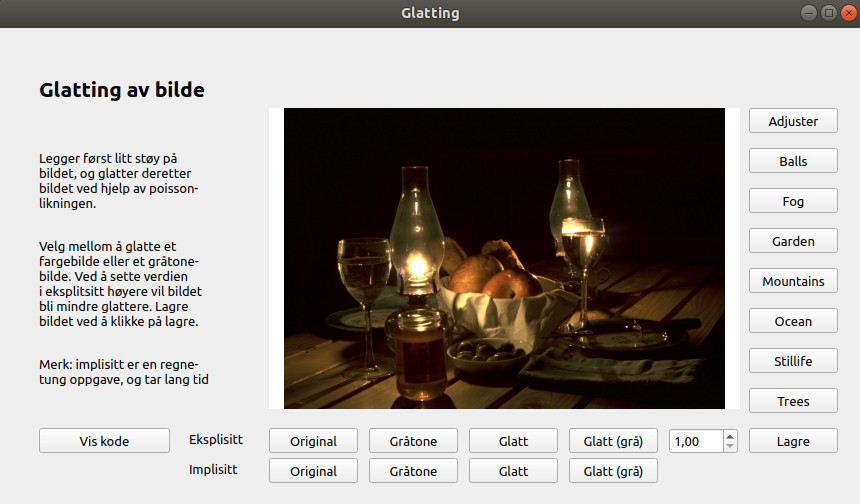
\includegraphics[width=0.5\columnwidth]{bilder/Gui/guiexample.jpg}
     \caption{Grafisk brukergrensesnitt - Glatting \label{fig:guiexample}}
\end{center}
\end{figure}

I hver modul importeres klassen \texttt{showCode(QMainWindow)}, som viser koden i et nytt vindu for implementasjonen. Koden som vises ligger lagret i en .txt-fil i \texttt{src/codes}, som vises ved å bruke funksjonen \texttt{FunctionGUI/ShowCode}. Her opprettes det et nytt \texttt{QMainWindow}, hvor koden vises i et rullbar tekstfelt. 

\subsubsection{Glatting}
Et bilde kan glattes ved å bruke en eksplisitt løsning av diffusjonslikningen. Dette gjøres av funksjonen \texttt{blurImage(self, colour)}. Denne henter først et fargebilde hvis colour er True eller gråtonebilde hvis colour er False. Videre lages en kopi av originalbilde som det legges litt støy på, før dette glattes ved å bruke funksjonen \texttt{eksplisittGlatting()} fra \texttt{Eksplisitt.py}. Tilslutt vises bildet ved å bruke modulens showImage-funksjon.

Bildet kan også glattes ved å bruke en eksplisitt løsning av diffusjonslikningen. Dette gjøres at funksjonen \texttt{blurImageImplsitt(self, colour=True)}. Hvis colour er True leses det inn et fargebildet, og hvis colour er False leses det inn et gråtonebilde ved bruk av \texttt{grayscale()} fra \texttt{Grayscale.py}. Disse bildene lagres som en numpyarray \texttt{u} som videre omformes til å inneholde verdier mellom 0 og 1, hvor verdier over 1 og under 0 klippes til lovlige verdier. Deretter glattes bildet \texttt{u} ved å bruke funksjonen \texttt{implisitt()} fra \texttt{implisitt.py}. Tilslutt vises bildet ved å bruke showImage-funksjonen i modulen.

\subsubsection{Inpainting}
I Inpainting sitt GUI er det mulig å få vist bildet med manglende informasjon. Dette gjøres ved å bruke funksjonen \texttt{showMask(self)}, som sender med \texttt{self.path} og tallet \texttt{2} til funksjonen \texttt{Inpaint()} i \texttt{Inpainting.py}. Denne funksjonen returnerer bildet med masken, som vises ved å bruke \texttt{showImage()} i modulen. Informasjonen i bildet fylles inn i funksjonen \texttt{inpaint(self)}, som sender med \texttt{self.path} og tallet \texttt{3} til \texttt{Inpaint()} fra \texttt{Inpainting.py}. Her returneres et bilde hvor informasjonen er fylt inn, som vises av \texttt{showImage()}. 

\subsubsection{Kontrastforsterkning}


\subsubsection{Demosaicing}


\subsubsection{Sømløs kloning}


\subsubsection{Konvertering av fargetone til gråtone}


\subsection{Anonymisering}


\subsection{Brukermanual}


\subsubsection{Glatting}


\subsubsection{Inpainting}


\subsubsection{Kontrastforsterkning}


\subsubsection{Demosaicing}


\subsubsection{Sømløs kloning}


\subsubsection{Konvertering av fargetone til gråtone}


Ta med til konklusjon: 
- gjort på nytt, droppet bruk av QtDesigner og heller skrevet alt i kode. Litt mer kontroll og lettere å justere visning av vinduer. Kunne da også enkelt implementert støtte for å kunne justere vinduer ved å dra i kantene
- droppet bruk av .ui-filer som hadde gjort det mye enklere å organisere prosjektet på en bedre måte
- En del cowboyløsninger når man bygger på og bygger på, spesielt lagring av bilder ble ganske rotete og unødvendig komplisert til slutt
- Mange steder som man kanskje burde laget GUI annerledes
